\documentclass{article}
\usepackage{tikz}
\usetikzlibrary{positioning, calc}

\begin{document}

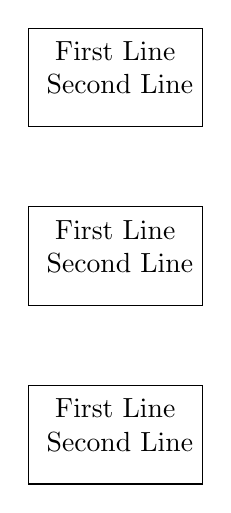
\begin{tikzpicture}[node distance=1cm]
    \node (node1) [draw] {%
        \begin{tabular}{@{}c@{}}
            First Line\\
            \vspace{0.5em} % Adjust vertical space as needed
            Second Line\\
        \end{tabular}
    };
    
    \node (node2) [draw, below=of node1] {%
        \begin{tabular}{@{}c@{}}
            First Line\\
            \vspace{0.5em} % Adjust vertical space as needed
            Second Line\\
        \end{tabular}
    };
    
    \node (node3) [draw, below=of node2] {%
        \begin{tabular}{@{}c@{}}
            First Line\\
            \vspace{0.5em} % Adjust vertical space as needed
            Second Line\\
        \end{tabular}
    };
\end{tikzpicture}

\end{document}